\documentclass[14pt, a4paper]{extreport}

% increase toc depth up to subsubsection
\setcounter{tocdepth}{3}
\setcounter{secnumdepth}{3}

\usepackage{tabu}
\usepackage{color}
\usepackage{array}
\usepackage{epstopdf}
\usepackage[russian]{babel}
\usepackage[utf8x, utf8]{inputenc}
\usepackage{tikz}
\usetikzlibrary{positioning, shapes.misc, shapes.geometric, arrows, shapes.multipart, shapes.arrows}
\usepackage{pgfplots}
\usepgfplotslibrary{dateplot}
\usepackage{amsmath}
\usepackage{algorithm2e}
\usepackage{algorithmic}
\usepackage{xcolor, colortbl}
\usepackage{mdframed}
\usepackage{textcase}
\usepackage{tabularx}
\usepackage[T2A,T1]{fontenc}
% 
\usepackage{indentfirst}
% setup  page fields
\usepackage{geometry}
\geometry{left=25mm}
\geometry{right=20mm}
\geometry{top=20mm}
\geometry{bottom=20mm}
% set line interval
\usepackage{setspace}
\onehalfspacing
% set footnotesize to 12 pt (for normalsize equal to 14 pt)
\renewcommand{\footnotesize}{\small}

\usepackage{titlesec}
\titleformat{\chapter}{\filcenter\bfseries}{\thechapter.}{1em}{}
\titleformat{\section}{\filcenter\bfseries}{\thesection}{1em}{}
\titleformat{\subsection}{\filcenter\bfseries}{\thesubsection}{1em}{}
\titleformat{\subsubsection}{\filcenter\bfseries}{\thesubsubsection}{1em}{}
\titleformat{\paragraph}{\filcenter\bfseries}{\paragraph}{1em}{}
\titlespacing*{\chapter}{0pt}{10pt}{10pt}

% make page number in top right corner
\usepackage{fancyhdr}
% rename abstract
\AtBeginDocument{\addto\captionsenglish{\def\abstractname{\MakeTextUppercase{Реферат}}}}
% counters
\usepackage[figure, table, page, enumiv]{totalcount}
%
\addto\captionsrussian
{
  \renewcommand{\contentsname}
    {\hfill{\normalsize\MakeTextUppercase{Содержание}}\hfill}
}
%
\addto\captionsrussian
{
  \renewcommand{\bibname}{\hfill\normalsize\MakeTextUppercase{Список использованных источников}\hfill}
}

\usepackage{tocloft}
% add dots for chapters
\renewcommand{\cftchapleader}{\cftdotfill{\cftdotsep}}
\renewcommand\cftchapfont{\mdseries}
\renewcommand\cftchappagefont{\mdseries}
% add dot after chapter number
\renewcommand{\cftchapaftersnum}{.}
%
\usepackage{caption}
\captionsetup[figure]{labelsep=space}
\captionsetup[table]{labelsep=space}

\usepackage{etoolbox}
\makeatletter
\patchcmd{\chapter}{\if@openright\cleardoublepage\else\clearpage\fi}{}{}{}
\makeatother

%
% flow chart commands
\tikzstyle{startstop} = [rectangle, rounded corners, minimum width=3cm, minimum height=0.5cm, text centered, draw=black, fill=red!30]
\tikzstyle{process} = [rectangle, minimum width=3cm, minimum height=0.5cm, text centered, draw=black, fill=orange!30]
\tikzstyle{decision} = [diamond, aspect=2, minimum width=1mm, minimum height=1mm, text centered, draw=black, fill=green!30]
\tikzstyle{arrow} = [thick,->,>=stealth]
%

% declare new operator for correct \limits usage
\DeclareMathOperator*{\argmin}{arg\,min}

\begin{document}
\RestyleAlgo{boxruled}
% style for top right corner page number
\fancypagestyle{plain}{%
    \fancyhf{} % clear all header and footer fields
    \fancyhead[R]{\thepage} % except the right top corner
    \renewcommand{\headrulewidth}{0pt} % remove line between header and main text
}
\pagestyle{plain}
\begin{titlepage}

\newpage

\begin{center}
Московский Авиационный Институт \\*
(национальный исследовательский университет) \\*

\vspace{2em}

Факультет прикладной математики и физики \\*
Кафедра вычислительной математики и программирования

\vspace{10em}

\Large \textbf{Курсовой проект \\*
по дисциплине <<Информационные технологии в проектировании и производстве>>} \\*

\vspace{3em}

<<Разработка проектного офиса <<Цифромед>>
\end{center}

\vspace{8em}

\hspace{25em}\vbox{
  \hbox{\bfseries{Выполнил:}}
  \hbox{\hspace{1em} Данилычев И.\,А.}
}

\vspace{2em}

\hspace{25em}\vbox{
  \hbox{\bfseries{Руководитель:}}
  \hbox{\hspace{1em} Скородумов С.\,В.}
}

\vspace{\fill}

\begin{center}
Москва, 2015
\end{center}

\end{titlepage}


\newpage
\vspace*{-25mm}
\tableofcontents
\newpage


\chapter{\MakeTextUppercase{Аннотация}}
При компании <<Скородумов и Партнеры>> был сформирован отдел проектирования программного обеспечения, специализирующийся на создании интернет-решений для малого и среднего бизнеса, образовательных учреждений, госпредприятий, задачей которого стала разработка офиса управления проектами, позиционирующегося как SaaS-приложение (Software as a Service, или <<ПО как услуга>>).

Результатом работы над проектом стало появление на свет проектного офиса <<Цифромед>>, представленного в виде веб-приложения, реализованного на языке Python с применением многофункционального фреймворка Flask.

Одной из целей проекта также являлось обеспечение компании <<Скородумов и Партнеры>> решением для управления проектами, предназначенным для внутреннего пользования и при этом, несмотря на имеющиеся аналоги (teamtools.ru, <<Мегаплан>> и др.), не уступающим им по основным показателям производительности и функциональности.


В данный отчёт входят:

\begin{itemize}
\setlength{\itemsep}{-1mm}
\item Иерархическая модель работ (WBS, Work Breakdown Structure) и бизнес-модель проекта;
\item IDEF0-модель цикла разработки данного проекта;
\item Техническое задание;
\item Структура базы данных приложения;
\item Анализ места размещения бизнес-логики;
\item Описание модели разработки;
\item Программная логика серверной части (backend);
\item Описание интерфейсной части (frontend);
\item Паспорт проекта и его данные.
\end{itemize}


\chapter{\MakeTextUppercase{Анализ проекта}}
\section{\MakeTextUppercase{Цель проекта}}

Ни для кого не секрет, что грамотное планирование в совокупности с тайм-менеджментом и распределением ответственности, зачастую реализуемым через методологию иерархической структуры проекта (Work Breakdown Structure), являются <<сердцем>> любого проекта и в основном определяют успешность его жизненного цикла вкупе с полнотой.

Целью данного проекта являлось создание веб-сервиса, оформленного в виде SaaS-решения и имеющего достаточно возможностей для замещения собой сторонних аналогов. Полученный продукт возможно как применять для внутреннего пользования, так и вывести на рынок ПО для последующей монетизации.

\subsection{\MakeTextUppercase{Достижимость цели}}
Несмотря на поставленную цель, проектная команда во главе с проект-менеджером отдаёт себе отчёт в том, что полученный результат может не содержать в себе всех заявленных особенностей, требуемых для успешной конкуренции со сторонними разработками. Более того, он может проигрывать по качеству исполнения и набору имеющихся или планируемых возможностей, которыми обладают коммерческие решения, созданные командами большого размера.
	
	
\section{\MakeTextUppercase{Продукт проекта}}

Для успешной реализации задач, поставленных в цели проекта, используется концепция проектного офиса, компонента, где происходит координация, обобщение информации и централизация прикрепленных проектов, ведется сводный мониторинг бюджетов и графиков. Проектный офис также обеспечивает коммуникацию между различными рабочими группами и скоординированную работу менеджеров проектов.

Проектный офис чаще всего, как и в данной работе, реализуется в виде Software as a Service-услуги, или, проще говоря, Web-приложения, не требующего установки на клиентские компьютеры. Всё, что требуется от членов проекта -- наличие доступа ко внутренней иерархии системы (комбинация логина и пароля), остальное же обеспечивается подразделением, ответственным за настройку и администрирование программных и аппаратных ресурсов организации.


\section{\MakeTextUppercase{Work Breakdown Structure}}
Work Breakdown Structure, или структура декомпозиции работ -- это иерархическое разбиение всей работы, которую необходимо выполнить для достижения целей проекта, на более мелкие операции и действия до такого уровня, на котором способы выполнения этих действий вполне ясны, а соответствующие работы могут быть оценены и спланированы. Она включает также определение промежуточных результатов всех составляющих эту структуру работ.

WBS чаще всего выполнена в виде древовидной диаграммы, корневым узлом в которой является сам проект, а его дочерними узлами -- результаты и подрезультаты, требуемые для достижения целей проекта. Важно отметить, что, помимо определения всего объёма работ для проекта, каждый из узлов структуры декомпозиции представляет собой объективный или как минимум измеримый результат.

Work Breakdown Structure используется для разделения ответственности и выделения конкретного набора обязанностей, которыми обладает каждая из рабочих групп и каждый сотрудник в отдельности. WBS для настоящего проекта приведена ниже:


\vspace{1em}

\begin{figure}[!htb]
  \centering
    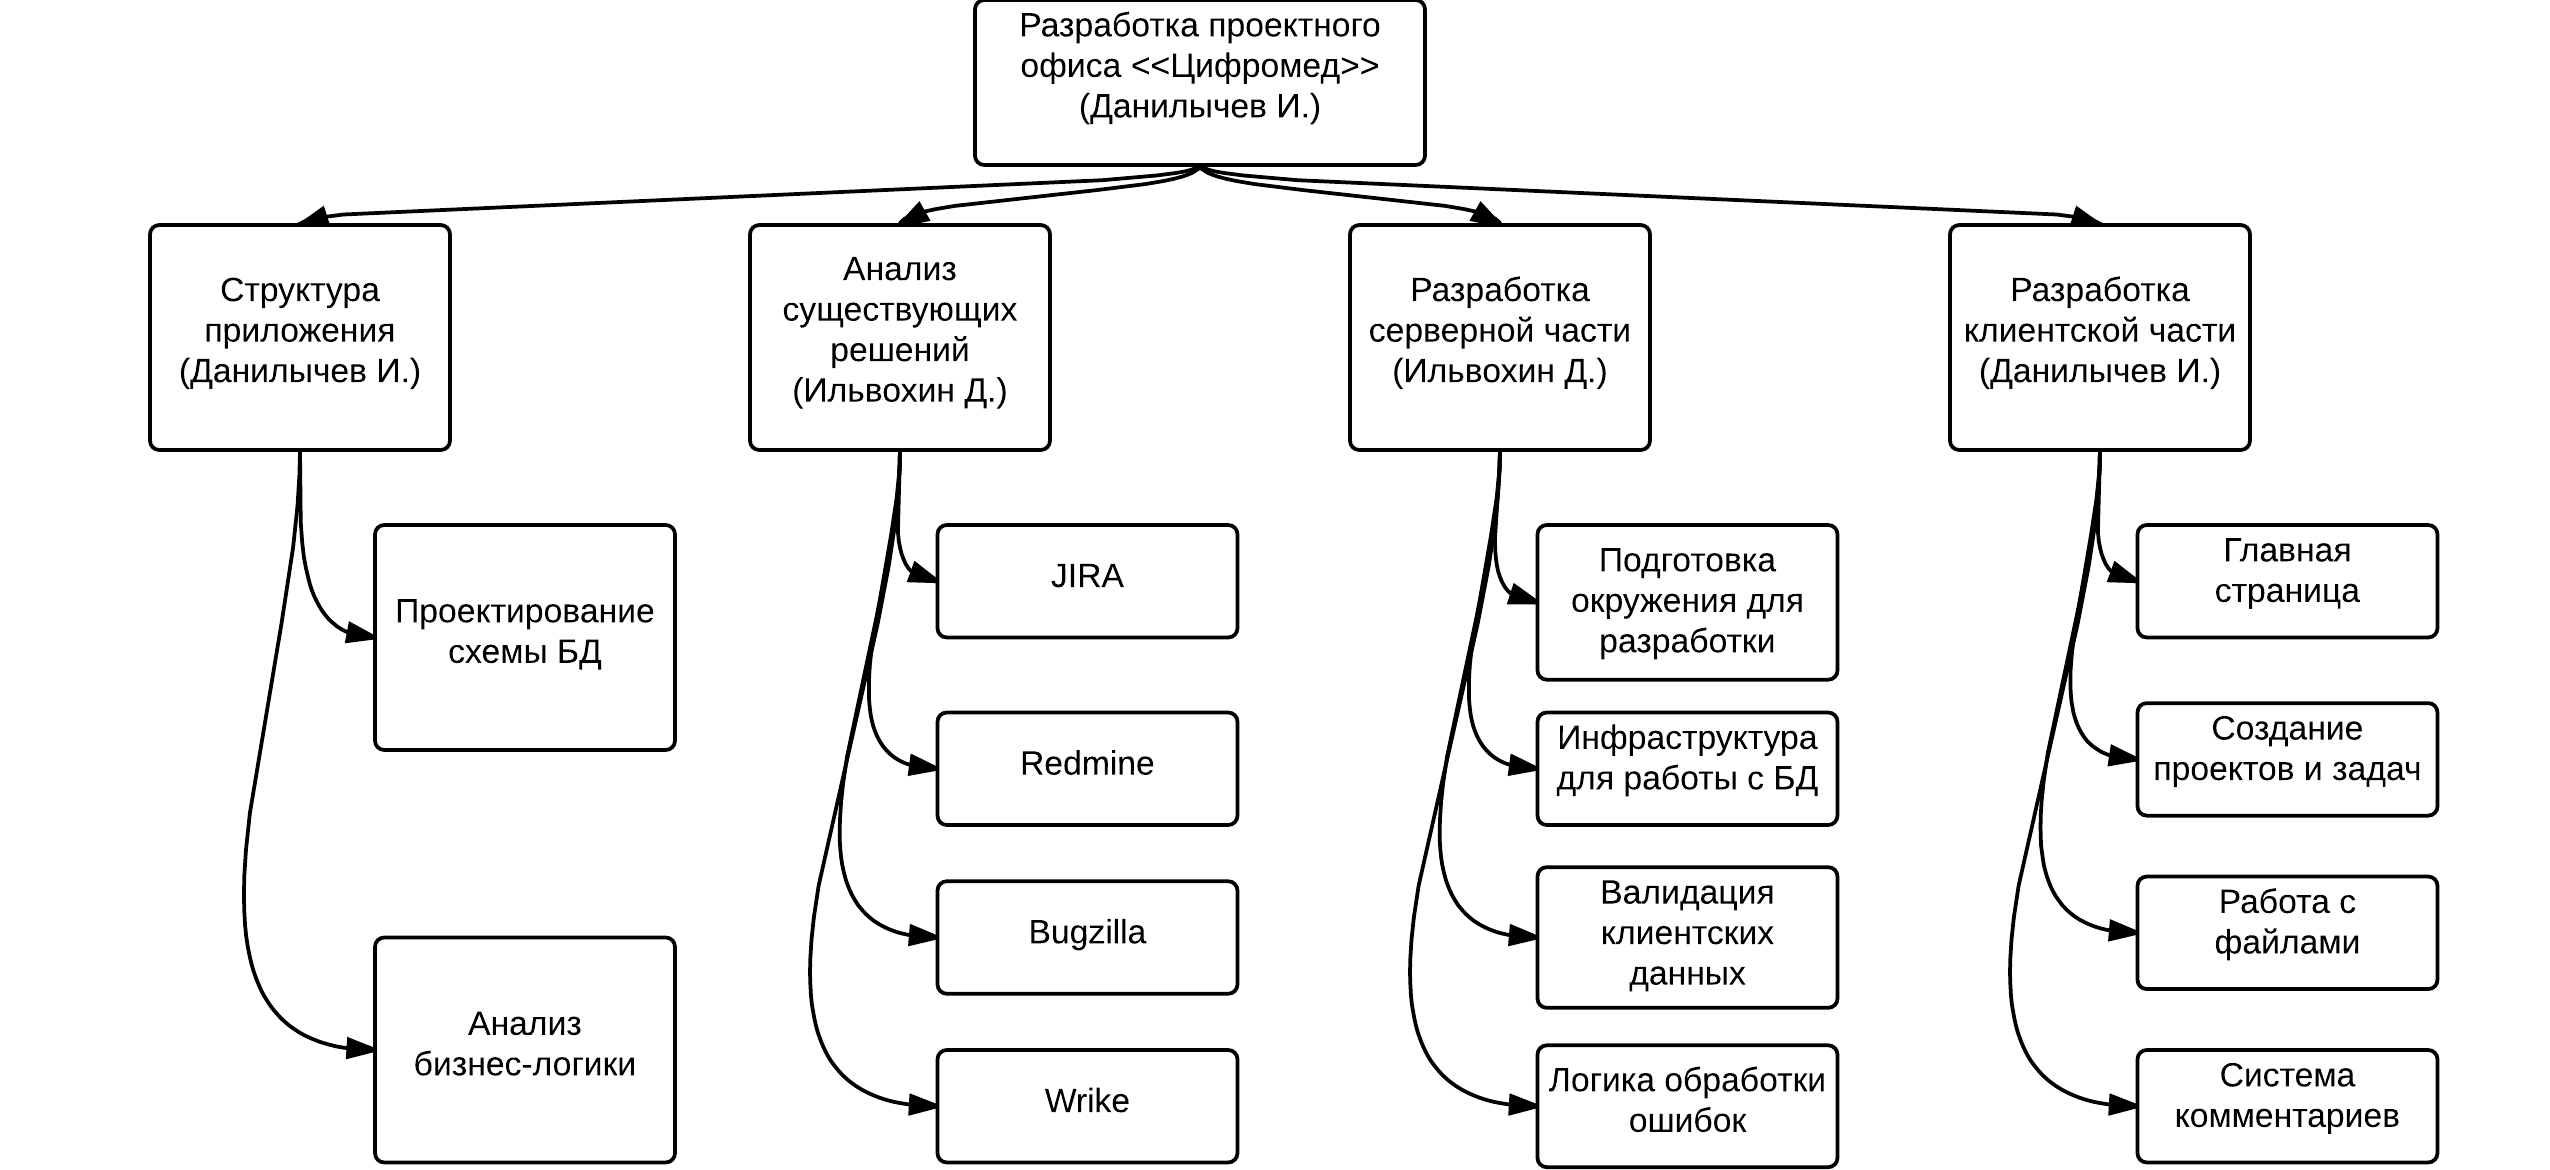
\includegraphics[scale=0.25]{../shared_images/wbs.png}
   \caption{Структура декомпозиции работ}
    \label{fig:start}
\end{figure}
\newpage


\section{\MakeTextUppercase{Бизнес-модель проекта}}

\begin{figure}[!htb]
  \centering
    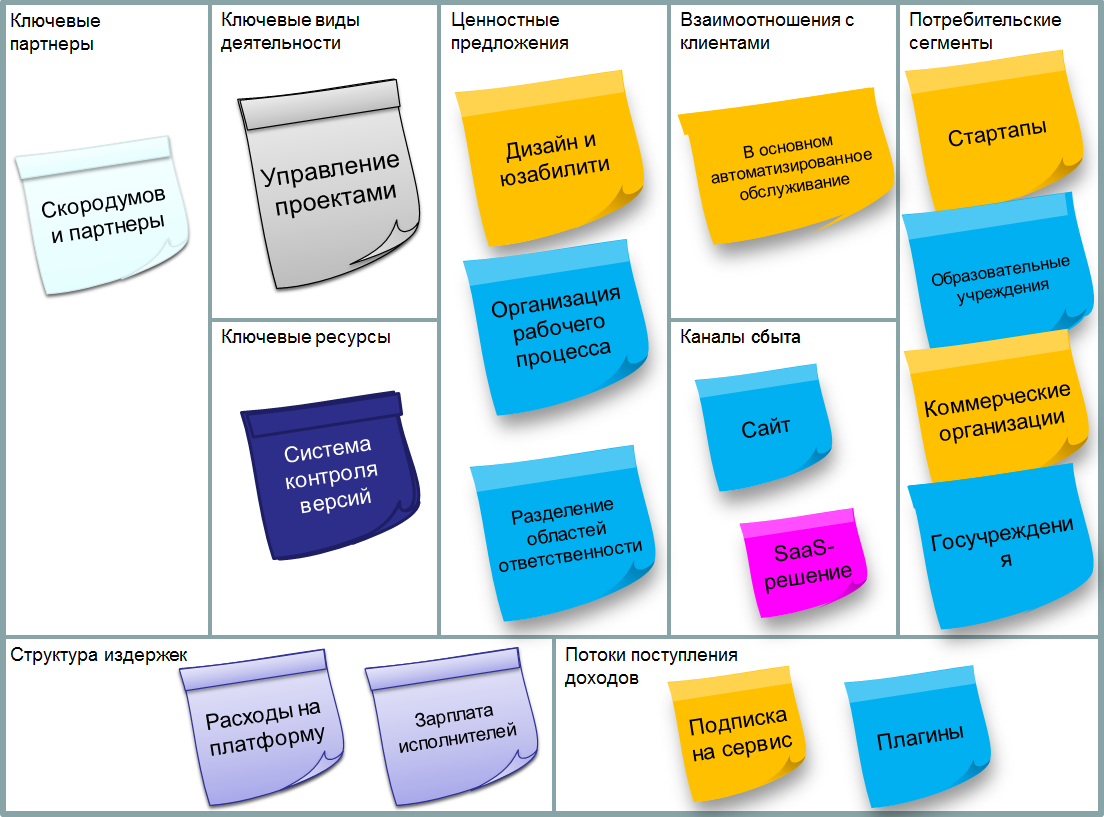
\includegraphics[scale=0.55]{../shared_images/business-model.png}
   \caption{Бизнес-модель проекта}
    \label{fig:start}
\end{figure}
  
Как видно из вышеприведённой модели, ключевым ресурсом проекта является децентрализованная система контроля версий. Её механизм контроля изменений, о котором будет рассказано в дальнейшем, позволяет параллельно разрабатывать несколько компонент приложения, попутно версионируя вносимые правки.

В потребительские сегменты попали коммерческие, государственные и образовательные организации, а также стартапы. Потребители (клиенты) – сердце любой бизнес-модели. Без (выгодных) клиентов не может существовать ни одна компания. Чтобы лучше удовлетворять нужды клиентов, желательно разбить их на группы по потребностям, особенностям поведения или иным признакам. Так, для образовательных организаций стоит делать упор на низкую себестоимость данного решения, его простоту в освоении, доступность и пр.

Взаимоотношения с клиентами, благодаря самобалансируемости и самоподдерживаемости проекта, сводятся к минимуму; что же касается сервиса поддержки клиентов, он относится к вопросам монетизации (поступление доходов).

Ценностные предложения сводятся к реализации функций, описанных в цели проекта: организации рабочего процесса и взаимодействия проектных команд и членов проектов, разделения сфер ответственности и т.д., а также простому, минималистичному дизайну, который в данном случае, учитывая порой переусложнённые интерфейсы конкурентов, является скорей положительным фактором.

Создание и воплощение ценностных предложений, поддержание взаимоотношений с потребителями, получение прибыли – все эти процессы связаны с какими-либо издержками. Расходы достаточно легко подсчитать при уже определённых ключевых ресурсах, видах деятельности. В данном случае издержки сводятся к оплате труда программистов, работавших над проектным офисом, и расходам на поддержание офиса в рабочем состоянии (оплата хостинга и т.п.)

Наконец, потоки поступления доходов в данной модели представлены двумя возможностями. Первая -- продажа подписки на сервис поддержки клиентов, который будет обеспечивать техническое функционирование офиса на клиентской стороне (аналогичный подход используется многими компаниями, поставляющими SaaS-услуги, напр., Redmine). Вторая -- разработка встраиваемых компонент, или плагинов, по техническому заданию заказчика, которому недостает в стандартной поставке решения некоторых возможностей.


\section{\MakeTextUppercase{IDEF0}}
IDEF0 -- методология функционального моделирования и графическая нотация, предназначенная для формализации и описания бизнес-процессов. Отличительной особенностью IDEF0 является её акцент на соподчинённость объектов. В IDEF0 рассматриваются логические отношения между работами без учёта временной последовательности; таким образом, описание workflow, или потока работ, остаётся за рамками данной модели.

\vspace{1em}

\begin{figure}[!htb]
  \centering
    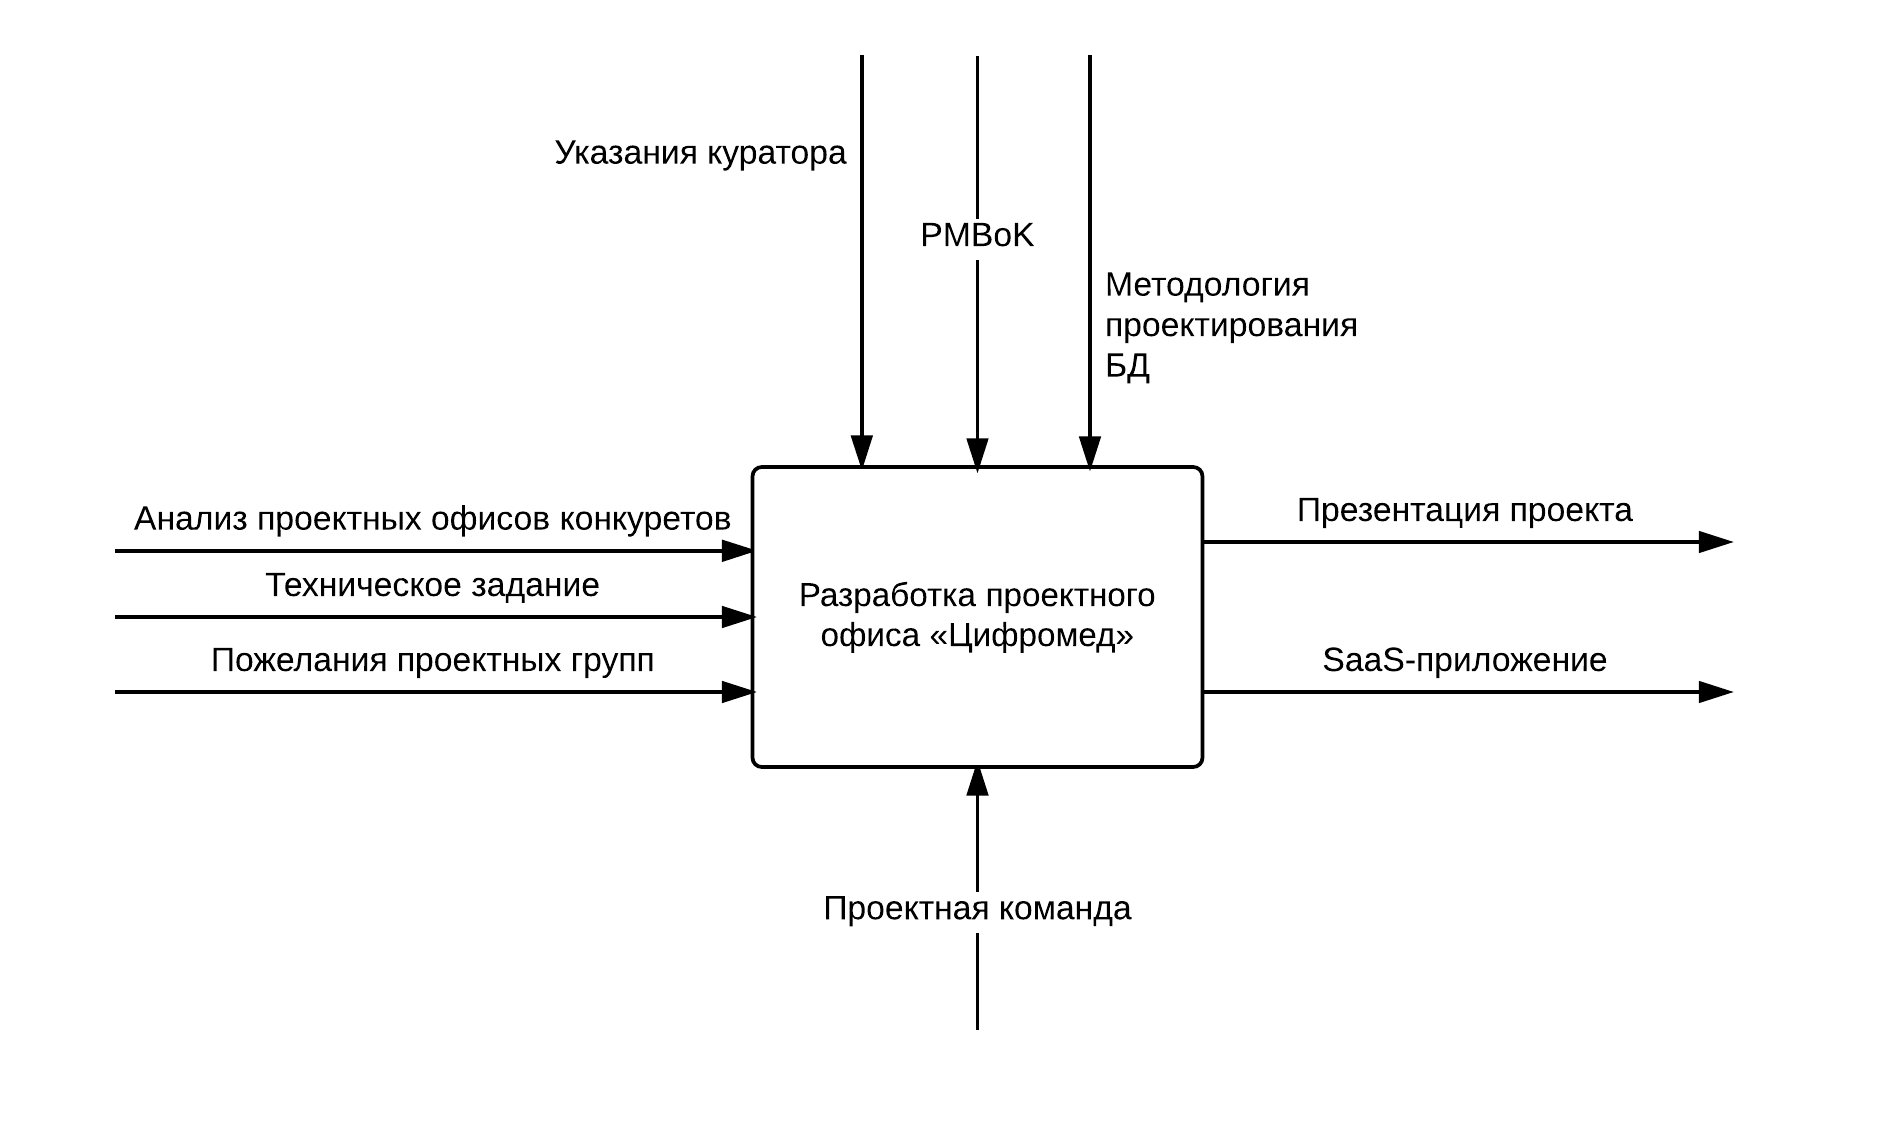
\includegraphics[scale=0.35]{../shared_images/idef0.png}
   \caption{IDEF0-диаграмма}
    \label{fig:start}
\end{figure}

Как видно из приведённой диаграммы, входными данными в настоящем проекте являются данные, полученные при анализе проектных офисов конкурентов, таких как JIRA, Redmine, Bugzilla, а также сформулированное самими разработчиками техническое задание, основанное на предъявляемых к системе требованиях. Кроме того, при разработке учитывались пожелания целевой аудитории, а именно -- проектных групп, являющихся потенциальными клиентами.

При разработке проектного офиса использовались указания куратора, Скородумова С.В., и материалы американского национального стандарта PMBoK, представляющего из себя сумму профессиональных знаний по управлению проектами.

Выходные данные представлены SaaS-приложением, реализующим онлайн-систему управления проектами (проектный офис), и презентацией получившегося продукта.

Декомпозированный уровень IDEF0 приведён ниже:

\vspace{1em}

\begin{figure}[!htb]
  \centering
    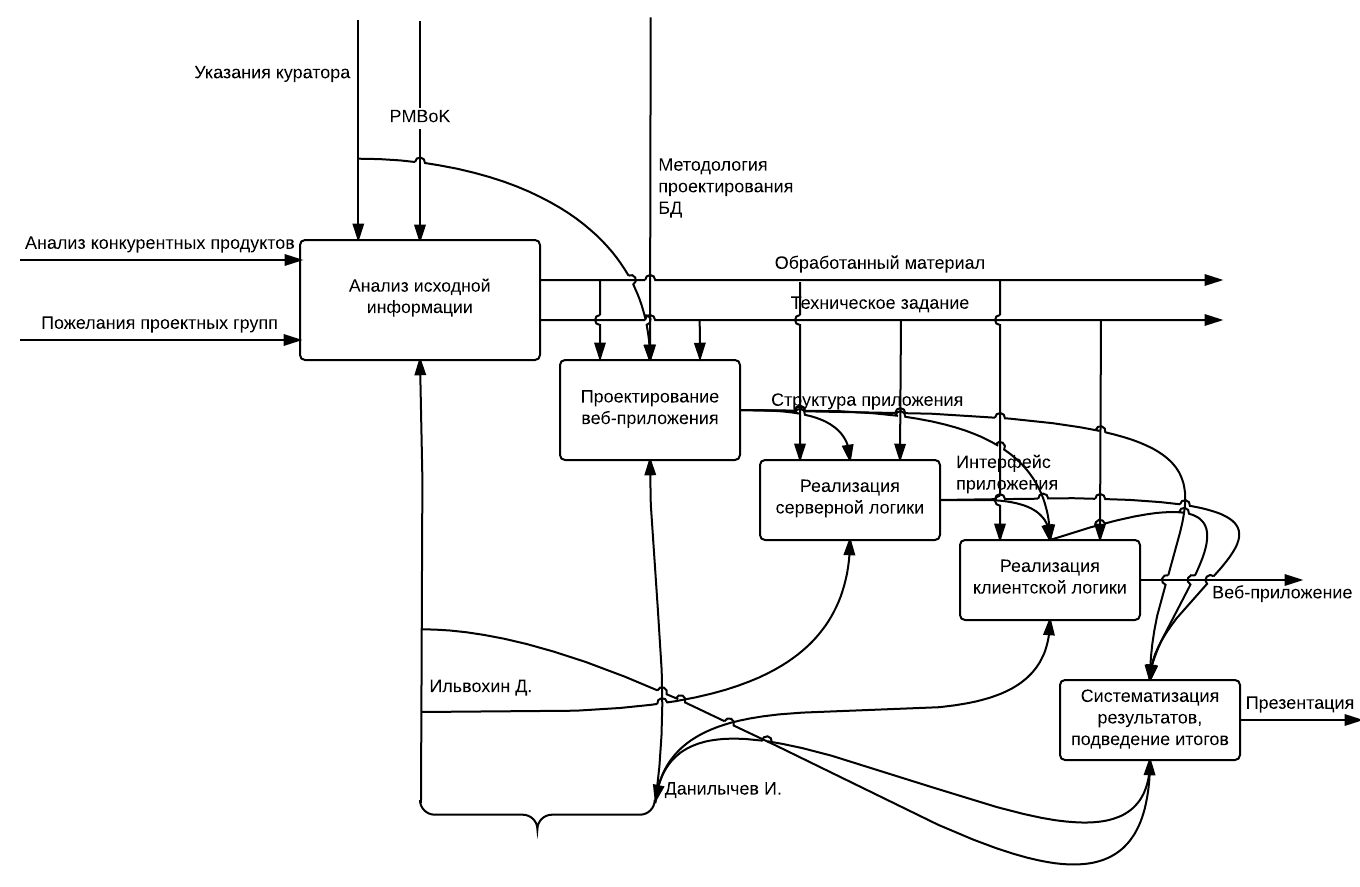
\includegraphics[scale=0.45]{../shared_images/idef0-decomposed.png}
   \caption{Декомпозированный уровень IDEF0}
    \label{fig:start}
\end{figure}

Из него видно, что после обработки конкурентных продуктов и пожеланий проектных групп появляются обработанный и систематизированный материал, который применяется во всех остальных стадиях жизненного цикла проекта, и техническое задание, служащее основой для построения схемы базы данных приложения и его общей системной структуры. Также оба компонента являются определяющими при реализации бизнес-логики на стороне клиента и сервера и применяются при подготовке финальной презентации, являющейся, в свою очередь, одним из продуктов проекта.


\chapter{\MakeTextUppercase{Проектирование приложения}}
\section{\MakeTextUppercase{Схема базы данных}}

\begin{figure}[!htb]
  \centering
    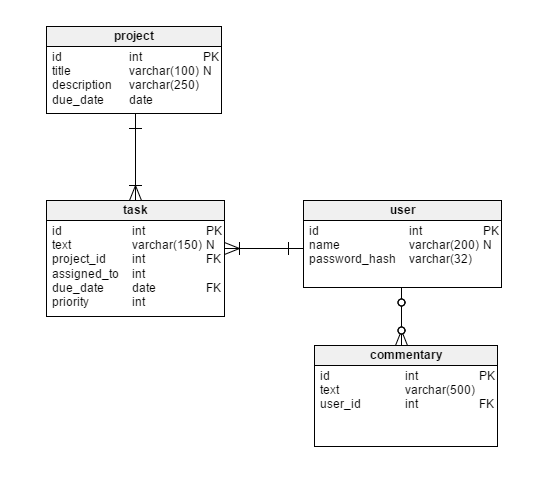
\includegraphics[scale=0.6]{../shared_images/schema.png}
   \caption{Схема БД}
    \label{fig:start}
\end{figure}

Как видно из схемы, ключевой сущностью является проект, который может иметь в своём составе одну или более задач. Задача, в свою очередь, связана с конкретным пользователем, ответственным за её сдачу, с помощью поля {\tt assigned\_to}.

У пользователей имеется возможность оставлять комментарии к задачам, используя реализованную на сайте систему комментариев. Каждый пользователь может как оставлять комментарии, так и не иметь их вообще.

Несмотря на произошедший позднее отказ от реляционных баз данных и переход к БД, основанных на технологии NoSQL, когда вся база представлена коллекцией документов различных типов без разбиения их на таблицы, спроектированная схема легла в основу финальной версии приложения.


\section{\MakeTextUppercase{Анализ места размещения бизнес-логики}}
\begin{figure}[!htb]
  \centering
    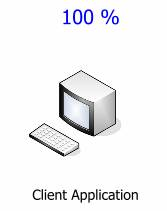
\includegraphics[scale=0.6]{../shared_images/business-logic/client.jpg}
   \caption{Клиентское приложение}
    \label{fig:start}
\end{figure}

На настольных приложениях бизнес-логика содержится на одном звене со всеми остальными слоями. Поскольку нет необходимости разделять слои, они зачастую перемешаны и не имеют четких границ.

\begin{figure}[!htb]
  \centering
    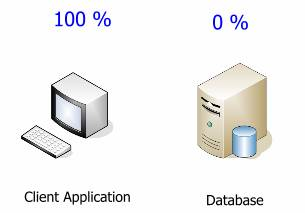
\includegraphics[scale=0.6]{../shared_images/business-logic/client-server.jpg}
   \caption{Приложение с архитектурой «клиент-сервер»}
    \label{fig:start}
\end{figure}


В клиент-серверном приложении имеются два звена, что приводит к созданию как минимум двух слоев. На начальном этапе сервер рассматривается только как удаленная база данных, и деление совпадает с рисунком -- приложение на клиенте и данные на сервере. Обычно вся бизнес-логика находится на клиенте, перемешанная с остальными слоями, такими как пользовательский интерфейс.

Достаточно быстро стало понятно, что можно сократить нагрузку на сеть и централизовать логику для уменьшения постоянных затрат на развертывание, перенеся большую часть бизнес-логики на сервер. Архитектурно сервер является хорошо подготовленным местом в клиент-серверной системе, хотя база данных как платформа даёт мало возможностей. БД были спроектированы для хранения и выдачи и в их архитектуру не были заложены возможности расширения в направлении бизнес-логики. Языки хранимых процедур в базах данных были разработаны для базовых преобразований данных, чтобы поддержать то, на что не хватало SQL. Языки хранимых процедур разработали для быстрого исполнения, а не для обслуживания сложных задач бизнес-логики.

Тем не менее, во избежание переусложнённости клиента часть бизнес-логики была перемещена в хранимые процедуры.

\begin{figure}[!htb]
  \centering
    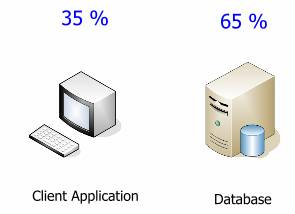
\includegraphics[scale=0.6]{../shared_images/business-logic/client-server-2.jpg}
   \caption{Часть логики хранится на сервере}
    \label{fig:start}
\end{figure}


Когда проблема клиент-серверной архитектуры стала явной, возросла популярность 3-х звенного подхода. Наибольшей и самой тяжелой проблемой того времени было количество подключений. Сейчас многие базы данных могут обрабатывать тысячи единовременных подключений, однако десятилетие или два назад большинство баз данных падало где-то на пятиста подключениях.

Стало популярным объединение подключений в пул, однако для реализации пула подключений в системе с множеством отдельных клиентов, необходимо внедрить третье звено между клиентом и сервером. Среднее звено так и стало называться «среднее звено». В большинстве случаев среднее звено существовало только для управления пулом соединений, но в некоторых случаях бизнес-логика начала перемещаться в среднее звено потому, что языки разработки (C++, VB, Delphi, Java) гораздо лучше подходили для реализации бизнес-логики, чем языки хранимых процедур. Вскоре стало очевидно, что среднее звено -- это наилучшее место для бизнес-логики, и схема приложения трансформировалась:

\begin{figure}[!htb]
  \centering
    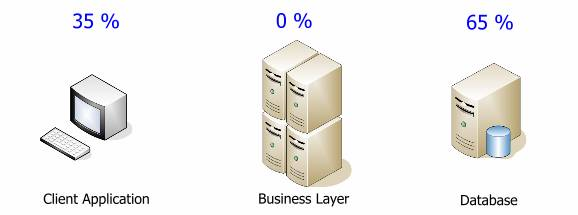
\includegraphics[scale=0.6]{../shared_images/business-logic/client-server-business.jpg}
   \caption{Пустой слой бизнес-логики}
    \label{fig:start}
\end{figure}

В таких случаях бизнес-слой не содержит бизнес правил. Это не настоящий бизнес-слой, а только форматтер XML (или другого потокового формата) и адаптер наборов данных базы данных. Хотя некоторые плюсы, такие как пул соединений и изоляция БД, могут быть достигнуты, это не настоящий слой бизнес-логики, скорее, инородный физический слой без слоя логики.

\begin{figure}[!htb]
  \centering
    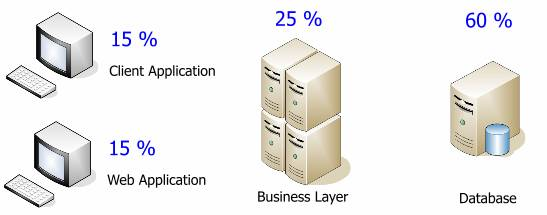
\includegraphics[scale=0.6]{../shared_images/business-logic/client-server-business-2.jpg}
   \caption{Слой бизнес-логики, частично разгружающий БД}
    \label{fig:start}
\end{figure}

Обычно некоторые бизнес-правила приложения переходят в бизнес-слой, но то, что было в базе данных, так в ней большей частью и остается. При повторном использовании бизнес-слоя в таких разработках бизнес-правила должны повторяться и в клиентском приложении. Это сводит на нет основную цель внедрения бизнес-слоя.

\begin{figure}[!htb]
  \centering
    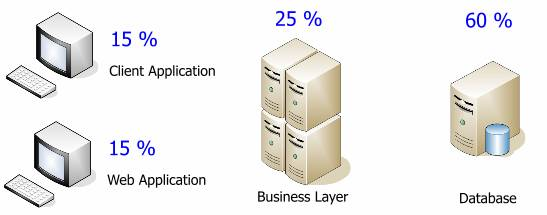
\includegraphics[scale=0.6]{../shared_images/business-logic/client-server-business-2.jpg}
   \caption{Полностью заполненный слой бизнес-логики}
    \label{fig:start}
\end{figure}

Тем не менее, идеальной моделью в данном случае является консолидированная модель, приведённая выше, когда вся бизнес-логика выделена из БД. Такая разработка имеет следующие преимущества:

\begin{itemize}
  \item Вся бизнес-логика находится в одном месте и может быть легко проверена, отлажена и изменена.
  \item Для реализации бизнес правил может быть использован нормальный язык разработки. В нашем случае таким языком стал Python, который больше подходит для данной задачи, чем SQL и хранимые процедуры.
  \item База данных становится слоем хранения и может заниматься эффективным получением и хранением данных без ограничений относящихся к слою бизнес-логики или представления.
\end{itemize}

Кроме того, основным преимуществом становится полное отделение от БД: вся работа с БД ведётся через адаптер, без привязки к конкретной технологии, будь то стэк Oracle или PostgreSQL. При необходимости могут быть составлены механизмы миграции, но бизнес-логика останется в неизменном виде. Как уже было сказано, это снимает лишнюю нагрузку с БД, что, в свою очередь, открывает широкие просторы для масштабирования:

\begin{figure}[!htb]
  \centering
    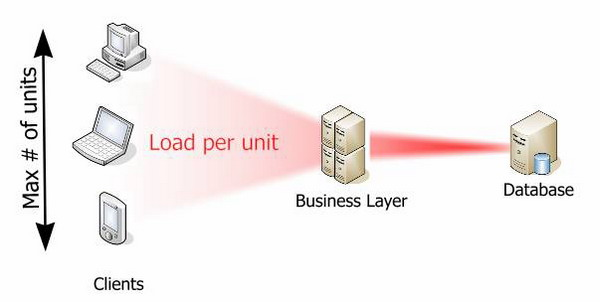
\includegraphics[scale=0.5]{../shared_images/business-logic/scaling.jpg}
   \caption{Поток данных и нагрузка}
    \label{fig:start}
\end{figure}

Перемещая вычисления в среднее звено, команда разработчиков отходит от границ слоя данных, что является несомненным плюсом: в то время как бизнес-звено имеет возможности масштабирования (можно закупить дополнительные сервера для обработки данных), попытка аналогичным образом увеличить количество серверов для хранения данных выльется в проблемы с дублированием, резервным копированием и -- возможно -- миграцией данных, что повлечёт замедление свежерасширенного слоя БД.


\chapter{\MakeTextUppercase{Сравнение существующих решений}}
Управление проектами --- в соответствии с определением национальным стандартом
ANSI PMBoK — область деятельности, в ходе которой определяются и достигаются
четкие цели проекта при балансировании между объёмом работ, ресурсами 
(такими как деньги, труд, материалы, энергия, пространство и др.), временем, качеством и рисками. 
Ключевым фактором успеха проектного управления является наличие чёткого заранее определённого плана,
минимизации рисков и отклонений от плана, эффективного управления изменениями.~\cite{wiki_pm}

\section{\MakeTextUppercase{Задачи программного обеспечения для управления проектами}}
Для достижения конечных целей проекта менеджеру проекта необходимо специальное программное обеспечение
для управления проектом или портфелем проектов.
Задачи программного обеспечения такого рода обычно делят на три части:
\begin{itemize}
  \item планирование;
  \item управление данными и предоставление информации;
  \item управление коммуникациями команды проекта.
\end{itemize}

\subsection{\MakeTextUppercase{Планирование}}
Одной из наиболее распространенных и на мой взгляд наиболее важных возможностей
программного обеспечения для управления проектами является возможность планирования
событий и управления задачами. Требования могут различаться в зависимости от того
для каких целей и проектов используется инструмент, наиболее распространенными являются:
\begin{itemize}
  \item планирование различных событий, зависящих друг от друга;
  \item планирование расписания работы сотрудников и назначение ресурсов на конкретные задачи;
  \item расчет времени, необходимого на решение каждой из задач;
  \item сортировка задач в зависимости от сроков их завершения;
  \item управление нескольким проектами одновременно.
\end{itemize}

\subsection{\MakeTextUppercase{Управление данными и предоставление информации}}
Программное обеспечение для управления проектами предоставляет большое количество
требуемой информации, такой как:
\begin{itemize}
  \item список задач и информацию распределения ресурсов;
  \item обзор информации о сроках выполнения задач;
\end{itemize}

\subsection{\MakeTextUppercase{Управление коммуникациями команды проекта}}
\begin{itemize}
  \item обсуждение и согласование рабочих вопросов проекта;
  \item предоставление доступа к информации о ходе проекта в виде живой ленты событий.
\end{itemize}

\section{\MakeTextUppercase{Типы программного обеспечения для управления проектами}}
Выделяют два типа программного обеспечения по размещению:
\begin{itemize}
  \item desktop (настольные);
  \item web-based (веб-приложения).
\end{itemize}

А также три типа по количеству пользователей использующих приложения:
\begin{itemize}
  \item персональные;
  \item однопользовательские;
  \item многопользовательские.
\end{itemize}

\section{\MakeTextUppercase{Сводная таблица}}
Для сравнения программного обеспечения для управления проектами было выделено
несколько пунктов:
\begin{enumerate}
\item Лицензия. Для использования приложения необходимо заплатить деньги
  его разработчикам, если это проприетарное программное обеспечение, как правило,
  при такой лицензии самостоятельная доработка продукта невозможна, потому
  что авторы приложения не распространяют его исходные коды или распространяют, но
  явно запрещают его изменение. При свободной лицензии,
  напротив, возможна самостоятельная доработка.
\item Язык реализации. У некоторых языков программирования, для больших приложений
  большой оверхед использования ресурсов, соответственно для развертывания приложения
  потребуется больше дорогих вычислительных мощностей.
\item Интерфейс. Чем больше возможностей доступа к приложению имеет пользователь, тем лучше.
  Удобство использования приложения --- первое, на что обращает внимание пользователь;
  в зависимости от своего впечатления, делает выбор в пользу какого-то приложения.
\item База данных. Нам, как разработчикам приложения, было интересно, на основе каких БД
  работают существующие/популярные системы, поэтому этот пункт тоже был включен в сравнительную таблицу.
\end{enumerate}

\begin{table}[!htb]
  \caption{Сравнение систем управления проектами~\cite{jira_off}~\cite{redmine_off}~\cite{bugzilla_off}~\cite{wrike_off}}
  \label{tab:cmp_pm}
  \begin{center}
    \begin{tabularx}{\textwidth}{|l|X|X|X|X|}
      \hline
      Система & Лицензия & Язык реализации & Интерфейс & БД \\
      \hline
      JIRA & проприетарное ПО & Java & Web, e-mail, RSS & MySQL, Oracle, PostgreSQL, MS SQL Server и др. \\
      \hline
      Redmine & GPL v2 & Ruby on Rails & Web, E-mail, Atom, iPhone, Windows Phone, Android & MySQL, PostgreSQL, SQLite \\
      \hline
      Bugzilla & MPL & Perl & Web, e-mail, RSS, Web service, cli, iPhone & MySQL, PostgreSQL \\
      \hline
      Wrike & проприетарное ПО & Java & Web, email & PostgreSQL \\
      \hline
      Цифромед & свободная & Python & Web & CouchDB \\
      \hline
    \end{tabularx}
  \end{center}
\end{table}

Для полноты сравнения в таблицу~\ref{tab:cmp_pm} добавлено приложение, разработанное нами.

\newpage

\chapter{\MakeTextUppercase{Подготовка окружения для разработки}}
Для совместной разработки проекта была выбрана децентрализованная система контроля
версий --- git, которая была создана Линусом Торвальдсом для управления разработкой
ядра Linux.~\cite{git_home}

Для разработки проекта было решено не поднимать git на собственном сервере, а использовать
готовую платформу Github. GitHub позволяет вносить в проект изменения, откатываться
к старым версиям, работать над одним и тем же кодом сразу нескольким независимым программистам,
ответвлять независимые ветки проекта и так далее

При разработке системы решили использовать модель разработки, предложенную Винсентом
Дрессэнем (англ. Vincent Driessen).~\cite{git_branching_model}

Основной идеей этой модели разработки является то, что все изменения происходят в
develop-ветке, от которой (когда разработка всех новых возможностей, которые
должны попасть в релиз закончена) отводится релизная ветка, изменения из которой
вносятся в master-ветку, которая считается стабильной в любой момент времени.
Более подробно модель разработки разобрана на рисунке~\ref{fig:branching}.

Пока мы находимся на ранней стадии разработки до версии 0.1, поэтому вносим все изменения
в master-ветку. % :D

\begin{figure}[!htb]
  \centering
    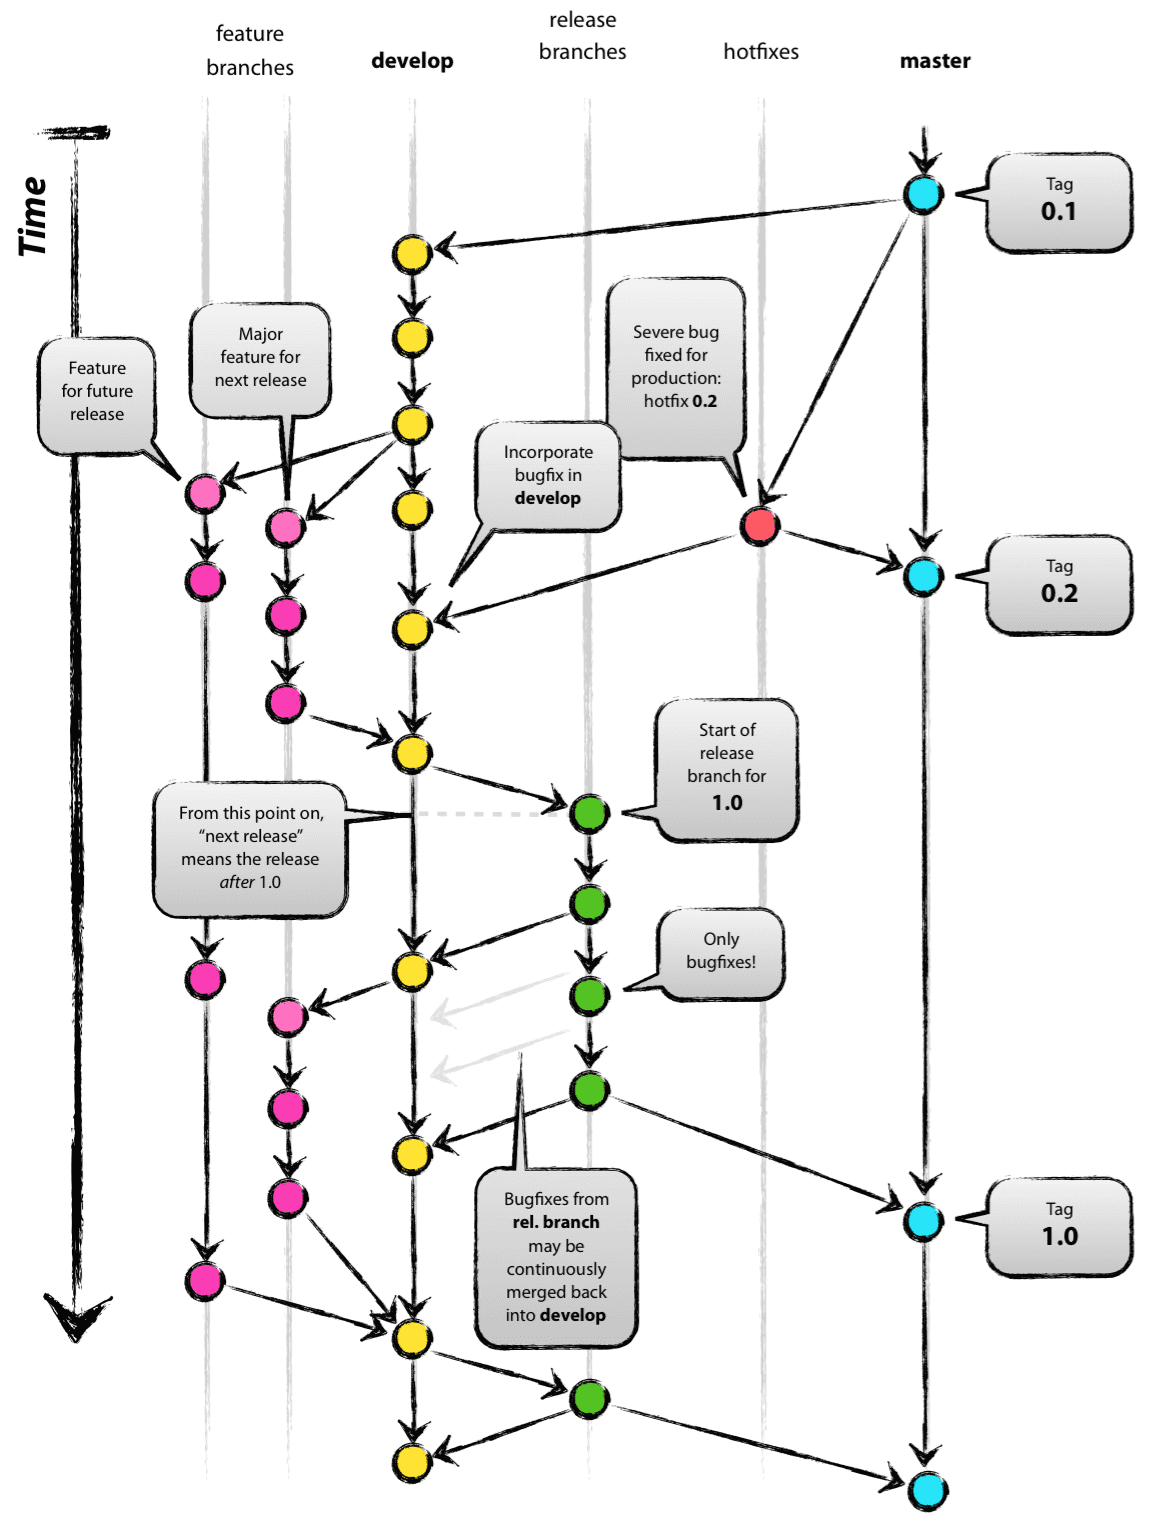
\includegraphics[scale=0.3]{../d/pics/branching.png}
    \caption{Модель разработки}
    \label{fig:branching}
\end{figure}


\chapter{\MakeTextUppercase{Разработка серверной части}}
Несмотря на то, что большинство существующих систем использует реляционные
базы данных, в своем проекте мы решили отказаться от традиционного подхода
к базе данных и использовать, современный, набирающий в последнее время популярность
NoSQL подход. NoSQL решения для управления большими данными используют гиганты индустрии,
такие как: IBM, Facebook, Netflix, EBay, Hulu, Yahoo!, благодаря поддержке которых технология
широко распространилась за последние несколько лет.

В разработке нашего решения для управления проектами мы использовали документоориентированную
систему управления базами данных Apache CouchDB.

Документоориентированные СУБД специально предназначены для хранения иерархических структур
данных (документов). В основе документоориентированных СУБД лежат документные хранилища (англ. document store),
имеющие структуру дерева (иногда леса).

Такой подход очень подходит для построения системы управления проектами, которая тоже имеет древовидную с структуру:
корень дерева --- проект, его узлы --- задачи, пример структуры приведен на рисунке~\ref{fig:project_tree}.

\begin{figure}[!htb]
  \centering
    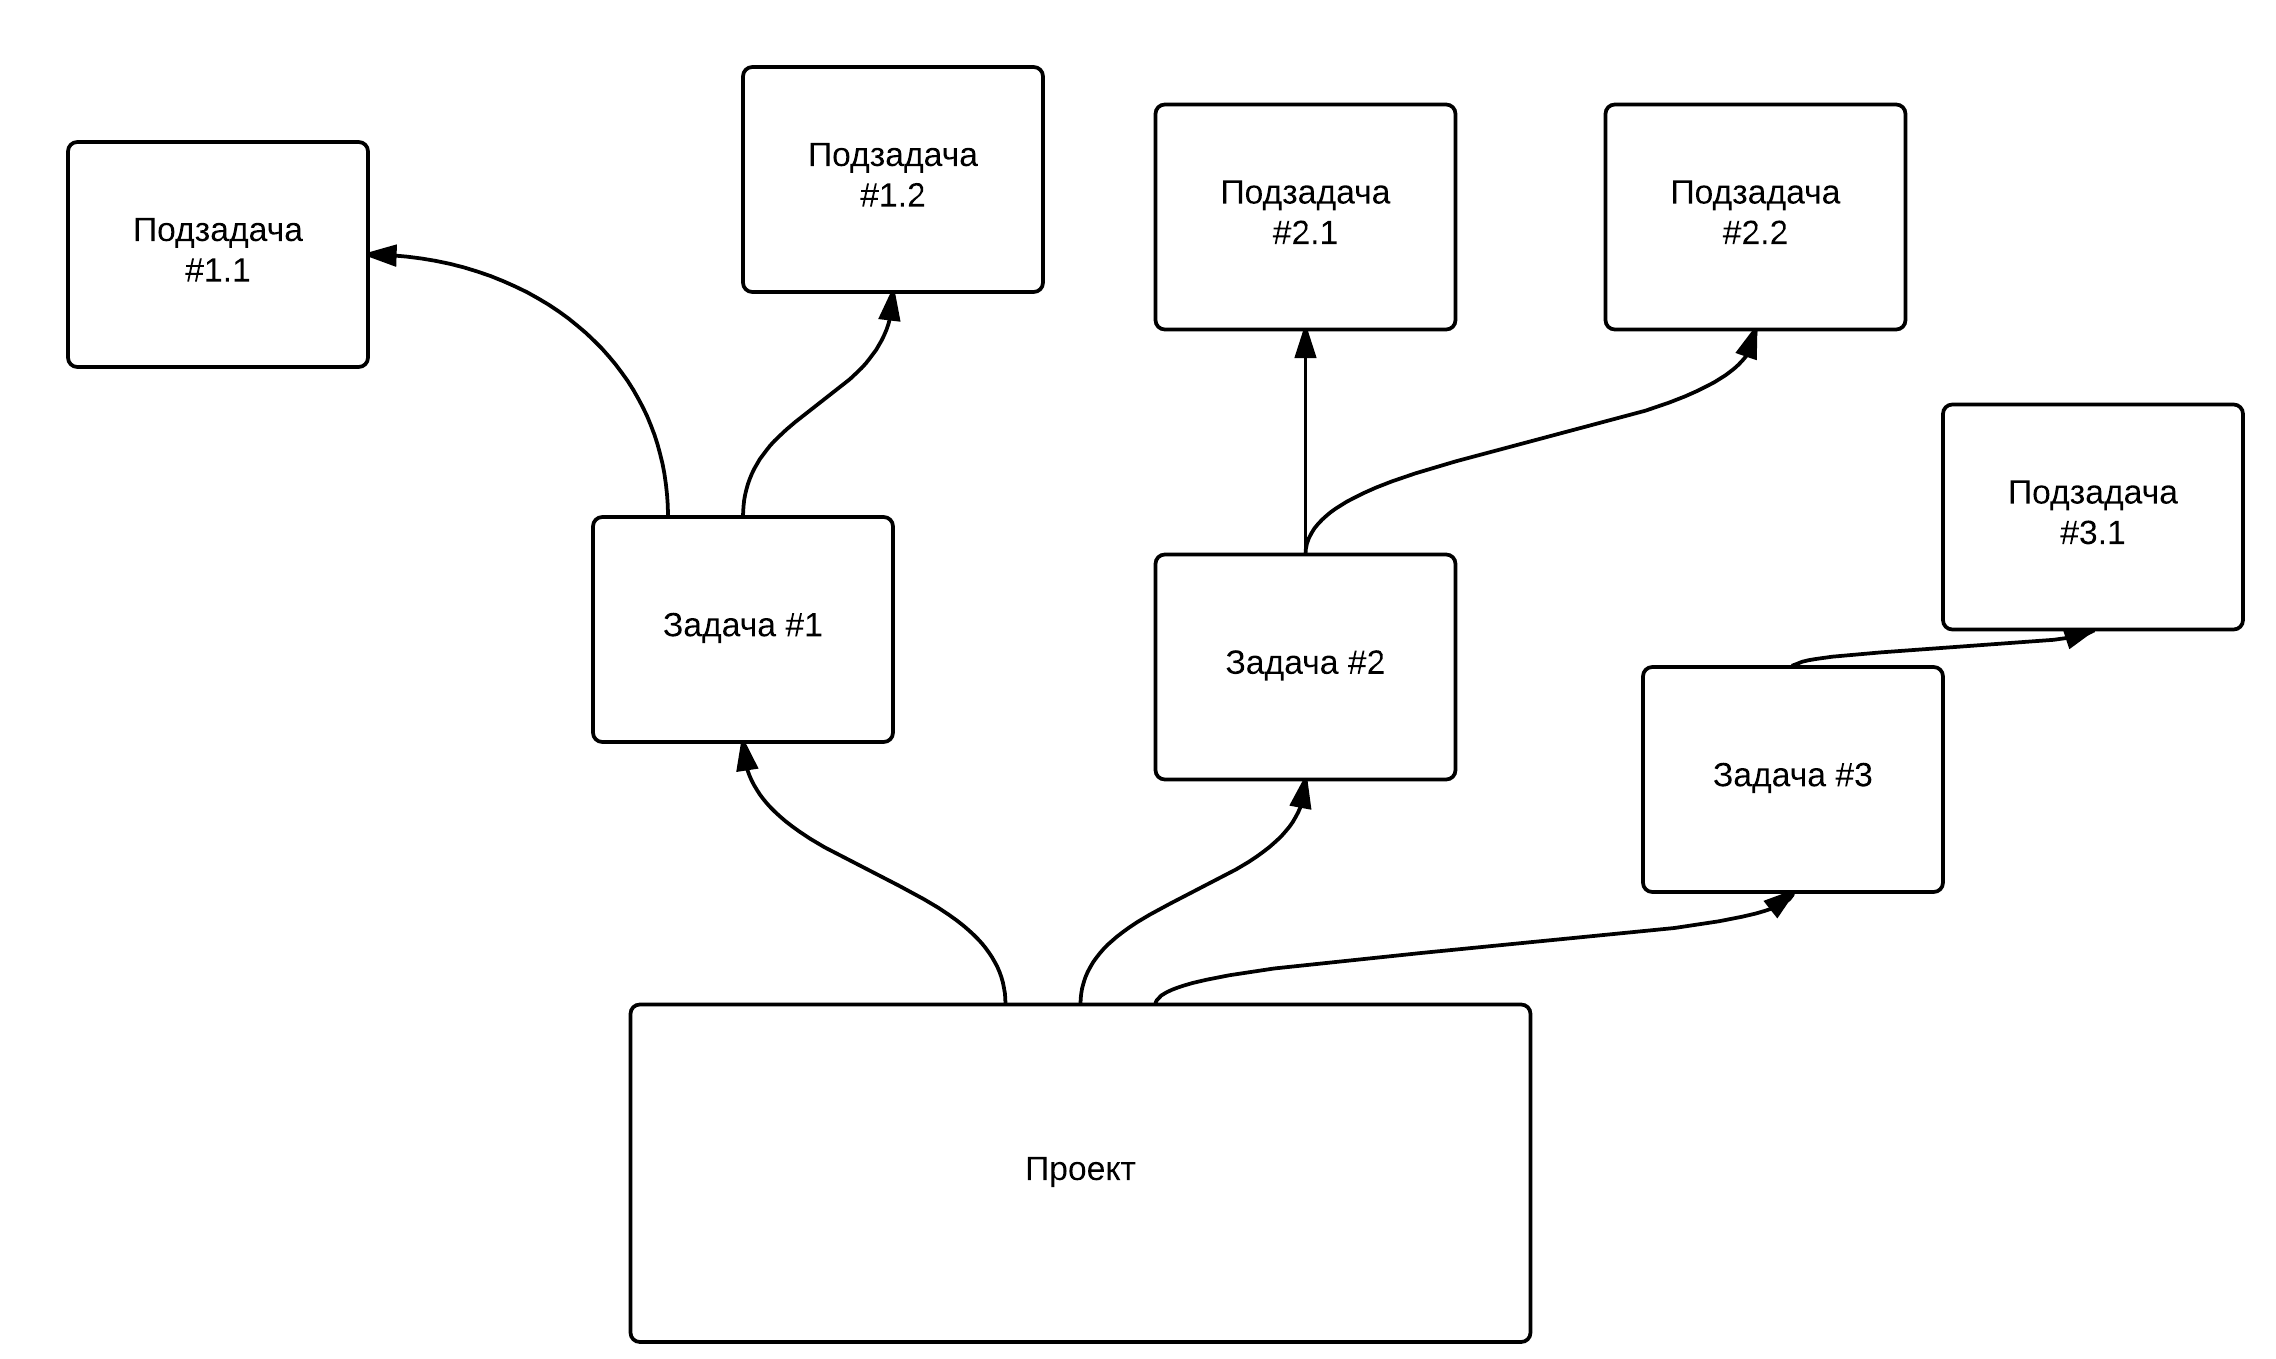
\includegraphics[scale=0.2]{../slides/images/test_tree.png}
    \caption{Структура проекта}
    \label{fig:project_tree}
\end{figure}

Для использования данных из CouchDB в коде приложения мы использовали технологию подобную ORM,
которая связывает базу данных с концепциями объектно-ориентированных языков программирования,
таким образом как бы создавая <<виртуальную объектную базу данных>>.

\newpage


\chapter{\MakeTextUppercase{Проектирование клиентской части}}
\section{\MakeTextUppercase{Главная страница}}
Первоначально на главной странице предполагалось выводить последние 10 созданных проектов, чтобы <<прорекламировать>> их остальным участникам и информационно насытить страницу, но поздней было принято решение не показывать ничего, кроме приглашения к логину. Сделано это было по причине того, что список проектов -- без возможности просмотра их незарегистрированным пользователем -- сам по себе не имеет никакого смысла; в результате при просмотре главной страницы незалогиненному пользователю предлагается залогиниться или зарегистрироваться.

\begin{figure}[!htb]
  \centering
    
\includegraphics[scale=0.8]{../shared_images/frontend/title-not-logged-in.png}
   \caption{Титульная страница глазами незарегистрированного пользователя}
    \label{fig:start}
\end{figure}

После логина вниманию пользователя предлагается три списка:

\begin{enumerate}
\item Список задач, в которых пользователь участвует (ответственен за их сдачу). Задачи отсортированы по крайнему сроку (deadline) и имеют, в зависимости от приоритета, различную окраску.
\item Список задач, созданных пользователем. Предназначен для менеджеров, следящих за активностью подчинённых.
\item Список проектов, созданных пользователем. Имеет то же значение, позволяя быстро просматривать задачи отдельного проекта и оценивать объём работы.
\end{enumerate}

\begin{figure}[!htb]
  \centering
    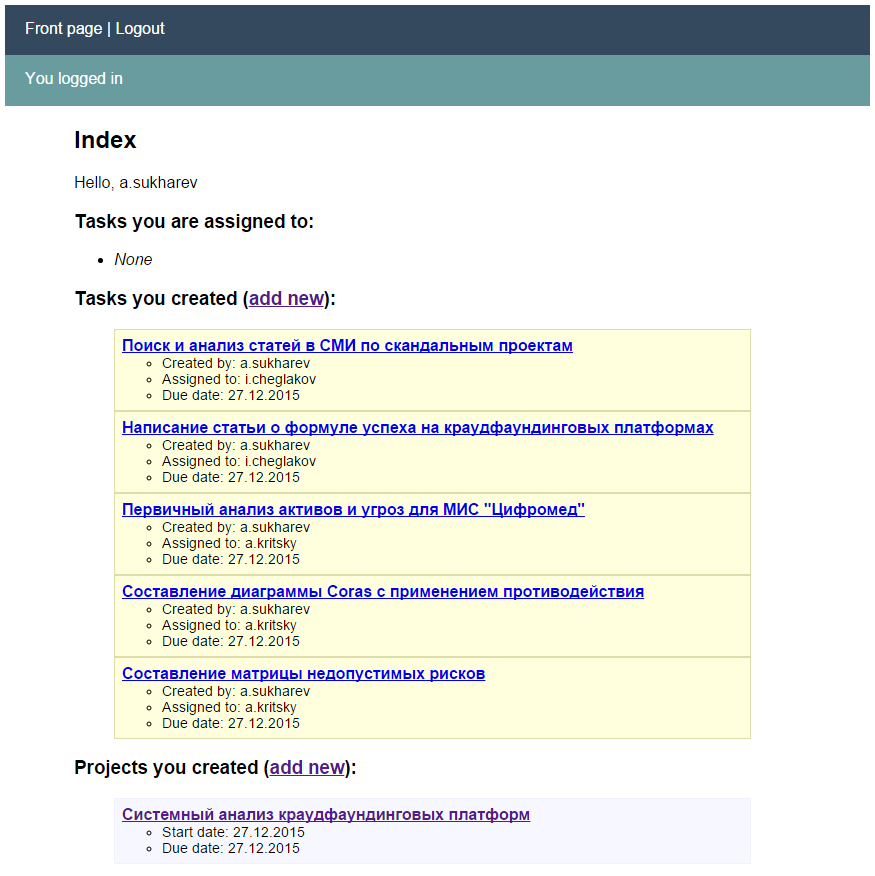
\includegraphics[scale=0.6]{../shared_images/frontend/title-logged-in.png}
   \caption{Титульная страница для участника или PM}
    \label{fig:start}
\end{figure}

\section{\MakeTextUppercase{Создание проектов и задач}}
Было решено воспользоваться успешно зарекомендовавшим себя интерфейсом вида <<Заголовок -- поле для заполнения>>. Отдельно стоит упомянуть, что через процедуру создания или редактирования к задаче можно добавить до трёх файлов, связанных с ней.

\begin{figure}[!htb]
  \centering
    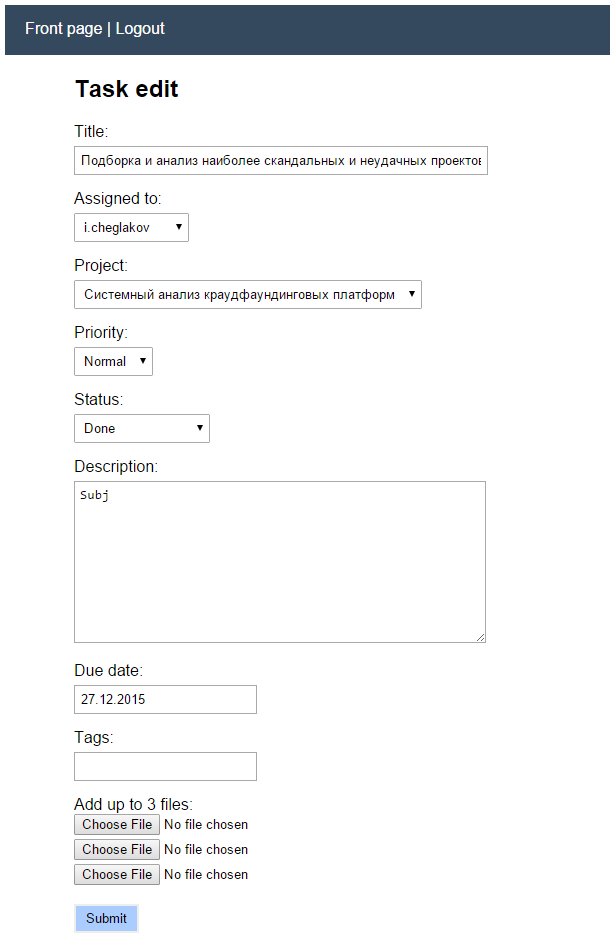
\includegraphics[scale=0.4]{../shared_images/frontend/task-edit.png}
   \caption{Форма редактирования задачи}
    \label{fig:start}
\end{figure}

\begin{figure}[!htb]
  \centering
    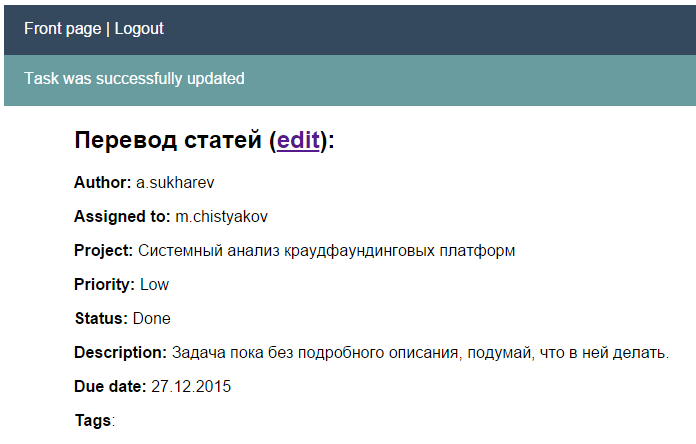
\includegraphics[scale=0.4]{../shared_images/frontend/task-view.png}
   \caption{Страница задачи}
    \label{fig:start}
\end{figure}

\section{\MakeTextUppercase{Работа с файлами}}

После информации о каждой задаче выводится список файлов, связанных с ней. По умолчанию файлы могут быть просмотрены любым человеком, имеющим ссылку. Тем не менее, ввиду сложности подбора ID (идентификационного номера) задачи, доступ извне к файлам затруднён. Данный принцип обеспечения безопасности называется security through obscurity, или <<безопасность через неясность>>. Его основная идея заключается в том, чтобы скрыть внутреннее устройство системы или реализацию для обеспечения безопасности.

\begin{figure}[!htb]
  \centering
    
\includegraphics[scale=0.75]{../shared_images/frontend/files.png}
   \caption{Список прикреплённых файлов}
    \label{fig:start}
\end{figure}

Стоит отметить, что неосторожный пользователь или злоумышленник не сможет затереть ранее залитый файл, поскольку при конфликте имён к имени нового файла добавляется случайный набор из 8 цифр и латинских букв. Типичная ссылка на файл в результате выглядит так: \\
{\tt http://127.0.0.1:1337/uploads/df0c17989df6268ec08cbc07e9962406/ \\
course-a1a70673.rar}

\section{\MakeTextUppercase{Система комментариев}}

Внизу каждой задачи имеется поле для оставления комментариев, а над ним -- список комментариев, отсортированный под дате добавления. Данная система позволяет осуществлять ведение дискуссий по теме задачи.

\begin{figure}[!htb]
  \centering
    
\includegraphics[scale=0.5]{../shared_images/frontend/comments.png}
   \caption{Комментарии к задаче}
    \label{fig:start}
\end{figure}



\chapter{\MakeTextUppercase{Выводы}}
Благодаря анализу существующих решений программного обеспечения для управления проектами, перед началом разработки, нам удалось выделить основные и самые востребованные в настоящее время возможности существующих продуктов и внести их в техническое задание, как обязательные для реализации в разрабатываемом нами приложении.

На основе выделенных требований было составлено техническое задание и была спроектирована схема базы данных, лёгшая впоследствии в основу архитектуры проекта. После детального анализа оптимального места размещения бизнес-логики для неё был выделен отдельный слой, что повлекло за собой отвязку проекта от реляционных БД и конкретных решений в принципе, добавляя приложению гибкости.

В рамках задачи подготовки рабочего окружения была развернута инфраструктура и выбрана модель разработки, которые использовались на протяжении всего процесса разработки приложения.

При разработке серверной части приложения была использована наиболее подходящая под нужды нашего проекта система управления базами данных, благодаря чему удалось существенно сократить время на написание кода для взаимодействия с базой данных и упростить процесс разработки. Также был спроектирован интерфейс приложения, состоящий из четырёх основных (не считая тривиальных) компонент, обеспечивающий удобную навигацию и ориентировку в списке имеющихся задач и их приоритетов.

Подводя итог, хотелось бы ещё раз отметить, что, несмотря на кажущуюся простоту получившегося решения, в нём была реализована вся заявленная в техническом задании функциональность; приложение обладает огромным запасом гибкости и является перспективным, но, к сожалению, не может конкурировать с плодами деятельности профессиональных разработчиков.

Тем не менее, результат проекта является приемлемой альтернативой известным проектным офисам, о чём свидетельствует тестирование, проведённое командой Сухарева А. В рамках данного тестирования проект-менеджером была воссоздана структура задач проекта и проведено разделение ответственности, а также протестирована система комментариев. Процесс упомянутого тестирования использован в качестве иллюстраций к разделу <<Проектирование клиентской части>>.

\newpage


\chapter{\MakeTextUppercase{Паспорт проекта}}
% Сырые PDF, экспортированные из MS Word; я не хочу перевёрстывать их в TeX
\newpage


\addcontentsline{toc}{chapter}{\MakeTextUppercase{Список использованных источников}}
\begin{thebibliography}{}
\bibitem{wiki_pm} Википедия [Электронный ресурс]: \\https://ru.wikipedia.org/wiki/Управление\_проектами
\bibitem{jira_off} Официальный сайт системы Atlassian JIRA [Электронный ресурс]: https://www.atlassian.com/software/jira
\bibitem{redmine_off} Официальный сайт системы Redmine [Электронный ресурс]: http://www.redmine.org
\bibitem{bugzilla_off} Описание возможностей на официальном сайте системы Bugzilla [Электронный ресурс]: https://www.bugzilla.org/features
\bibitem{wrike_off} Документация на официальном сайте системы Wrike [Электронный ресурс]: https://developers.wrike.com/documentation/api/overview
\bibitem{git_home} Домашняя страница Git [Электронный ресурс]: http://git-scm.com
\bibitem{git_branching_model} A successful Git branching model By Vincent Driessen [Электронный ресурс]: http://nvie.com/posts/a-successful-git-branching-model
\bibitem{} Википедия [Электронный ресурс]: \\https://ru.wikipedia.org/wiki/Бизнес-логика
\bibitem{} Chad Z. Hower ``Dude, where's my business logic?'' [Электронный ресурс]: http://www.codeproject.com/Articles/10746/Dude-where-s-my-business-logic
\bibitem{} Руководство по проектированию реляционных баз данных [Электронный ресурс]: http://habrahabr.ru/post/193136/
\bibitem{} Глеб Арестов <<Три правила проектирования интерфейсов>> [Электронный ресурс]: http://habrahabr.ru/post/211659/
\end{thebibliography}

\end{document}
